\section{Durchführung}
\label{sec:Durchführung}
Abbildung \ref{fig:waermepumpebildkonkret} zeigt die konkrete, hier verwendete
Messapparatur. Das hier verwendete Transportgas ist Dichlordifluormethan
\ce{CCl2F2}.
\begin{figure}
  \centering
  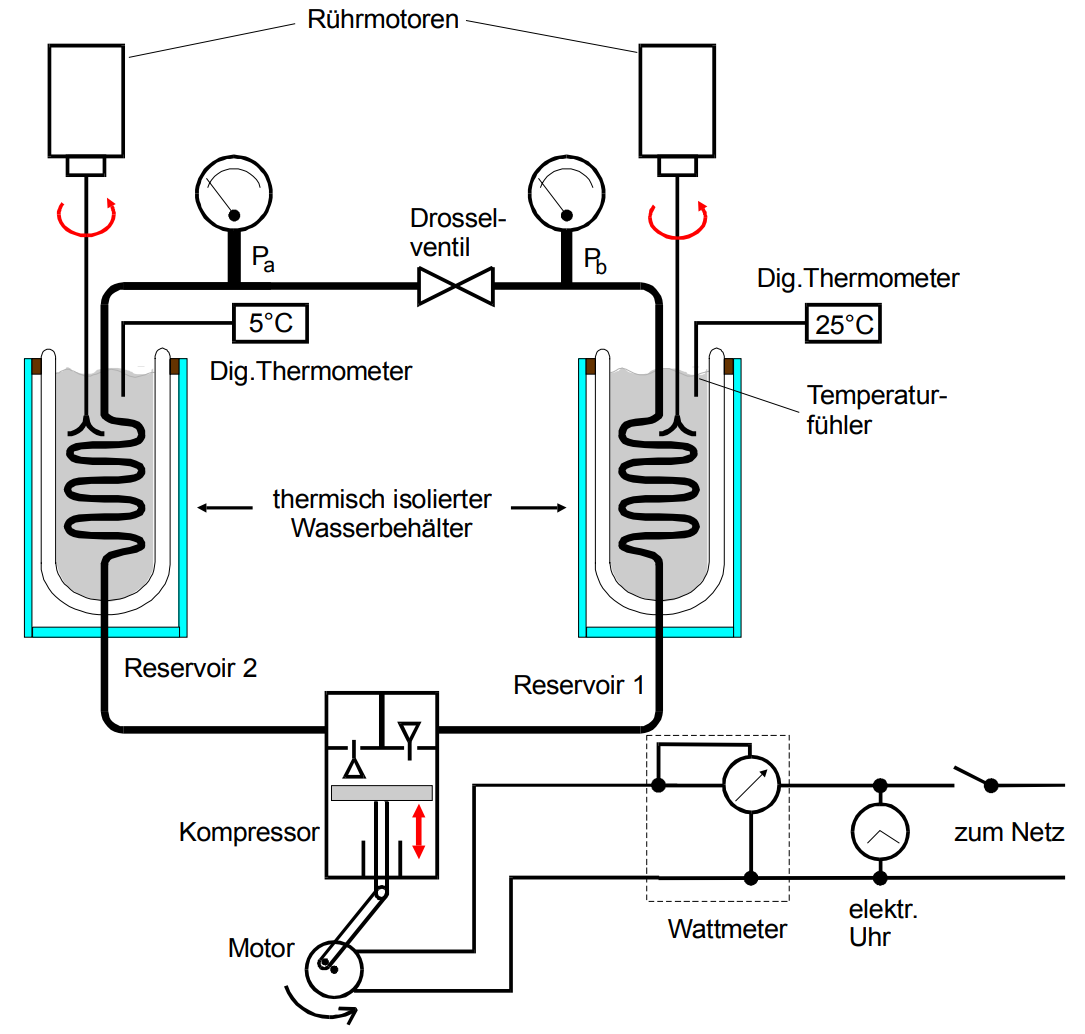
\includegraphics[width=300pt]{data/waermepumpekonkret.png}
  \caption{Skizze der Apparatur zur Versuchsdurchführung \cite{Versuchsanleitung}.}
  \label{fig:waermepumpebildkonkret}
\end{figure}
Zu Anfang werden jeweils vier Liter Wasser in die beiden Eimer gegeben, die die
Wärmereservoire darstellen. Um den Versuch zu beginnen, wird der Kompressor eingeschaltet.
Die Temperaturen $T_\text{kalt}$ und $T_\text{warm}$, die Drücke $p_\text{kalt}$
und $p_\text{warm}$ und die Leistungsaufnahme des Kompressors werden in Abhängigkeit der
Zeit gemessen. Die Aufnahme der Werte geschieht im Abstand von einer Minute. Um die
Stoffe in den Reservoirs angemessen zu durchmischen, rühren zwei auch in der Skizze dargestellte
Rührmotoren das Wasser ständig um. Die Messreihen werden aufgenommen, bis die Temperatur
$T_\text{warm}$ circa $\SI{50}{\celsius}$ beträgt. Ist dies der Fall, wird der Kompressor
abgeschaltet und damit die Durchführung des Versuchs beendet.
